\chapter[EXEMPLO DE USO]{EXEMPLO DE USO}
\label{chapter:example}

Como forma de ilustração de uso do serviço que desenvolvemos elaboramos uma
aplicação que chamamos de Forensic, que interage com o Shock via Kafka,
respeitando as definições feitas à cerca da API. A aplicação foi feita em
Elixir, uma linguagem funcional desenhada para construir aplicações
manuteníveis e escaláveis, utilizando o \textit{framework} Phoenix, que
facilita no desenvolvimento de aplicações Web.

O Forensic tem como principais objetivos abstrair o Shock do usuário final,
e consequentemente, as ferramentas de Big Data (como o Spark), ao passo em que
fornece um conjunto de funcionalidades que permitem ao usuário final configurar
a atuação dos \textit{streams}, semelhante a outros serviços existentes,
como o Amazon AWS\footnote{\url{https://aws.amazon.com/kinesis/analytics/}}.
Um usuário que deseje interagir com o Shock e InterSCity deve então:
(i) configurar um \textit{stream} novo com os
parâmetros desejados; (ii) criar esse \textit{stream} no Shock; (iii) injetar
esse \textit{stream} no Shock; (iv) e iniciar o processamento do
\textit{stream}.

De maneira geral, o Forensic espelha as abstrações do Shock (como os
\textit{streams}) e apresenta outras. Um dos conceitos necessários para o
uso efetivo da aplicação é o entendimento da arquitetura de camadas
\textit{ingest, store, analyze} e \textit{publish}, apresentada na Figura
\ref{fig:ingeststore}, que criamos para o Forensic. Essa arquitetura é baseada
em arquiteturas mais difundidas, como a \textit{ingest, store, analyze} e
\textit{visualize}, utilizada na plataforma Google Cloud
Platform\footnote{\url{https://cloud.google.com/solutions/data-lifecycle-cloud-platform}},
e a arquitetura \textit{collecton tier, message queuing tier, analysis tier,
in-memory data store} e \textit{data access tier}, explicada em
\citeonline{psaltis2017streaming}. O Forensic usa a abstração de \textit{stages}
para implementar a arquitetura mencionada, de modo que cada \textit{stage}
representa um passo da arquitetura. Um \textit{stream} têm então no máximo
4 \textit{stages}, e caso um necessite de mais, novos \textit{streams} devem
ser criados, e o resultado de um \textit{stream} deve ser utilizado como entrada
em outro.

O Forensic se comunica com o Shock via Kafka através de uma API que se assemelha
ao padrão JSON. Essa API utiliza o padrão ``arg1;\{arg2\}'',
onde o primeiro \textit{token} (antes do ponto e vírgula), ``arg1'', representa o nome
da ação desejada, e o segundo, ``arg2'', os argumentos da ação. Um
\textit{handler} no Shock receberá a ação requisitada no método
\textit{handle}, e deve tratar a requisição recebida. Por exemplo, uma mensagem
\textbf{ingestion;\{"stream": "mystream", "shock\_action": "socketIngestion"\}},
deve ser enviada caso queira-se o registro de um estágio de ingestão no
\textit{stream} \textit{mystream} via a função \textit{socketIngestion}.

\begin{figure}
  \centering
  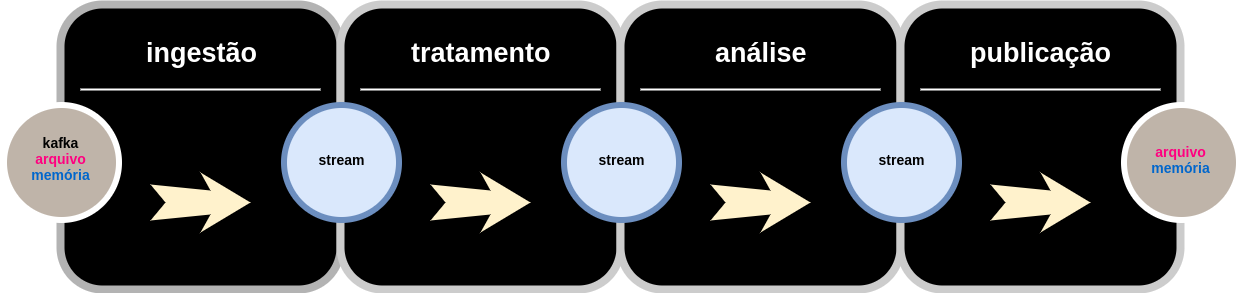
\includegraphics[width=\textwidth]{figuras/arquiteturaforensic.png}
  \caption{Padrão \textit{ingest, store, analyze e publish.}}
  \label{fig:ingeststore}
\end{figure}

O primeiro estágio de um \textit{stream}, \textit{\textbf{ingest}}, trata-se da
ingestão dos dados a partir de alguma fonte, como algum tópico do Kafka, ou
algum arquivo novo. Atualmente o Shock fornece três tipos diferentes de
ingestão: ingestão via tópico do Kafka, ingestão via arquivo (Parquet e Json)
e ingestão via \textit{socket}. A depender da estratégia de ingestão, alguns
parâmetros são necessários na configuração - numa ingestão via Kafka, por
exemplo, é necessário configurar o endereço do
\textit{broker} e os tópicos que serão utilizados. Ao final, o Forensic deve
passar os parâmetros configurados para o \textit{stream}, espelhando as
funcionalidades do Shock para o usuário final. A Figura \ref{fig:forensicparams}
apresenta a página de configuração de parâmetros no Forensic para uma ingestão
via Kafka.

\lstinputlisting[caption={
  Ingestão de dados no Shock via \textit{socket} e Kafka. Disponível em
  \url{https://gitlab.com/DGuedes/shock/blob/master/shock/ingestion.py}.
}]{editaveis/arquivos/ingestion.py}

\begin{figure}
  \centering
  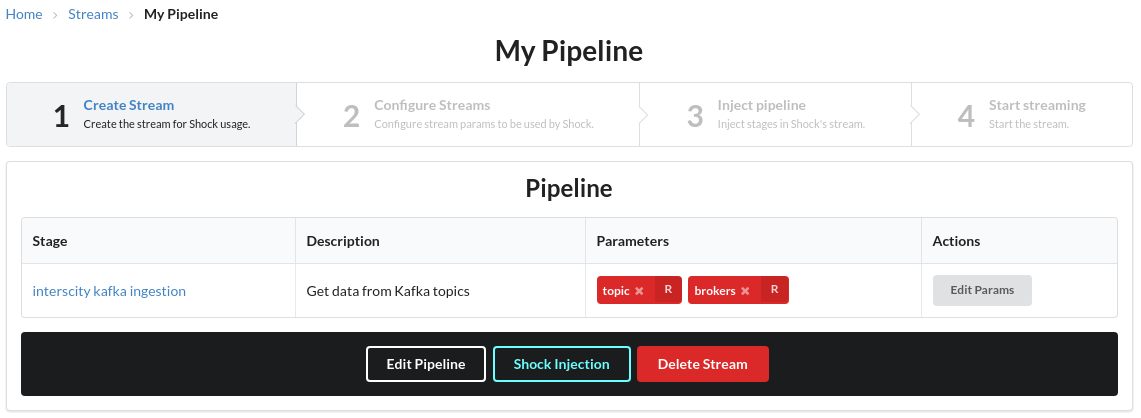
\includegraphics[width=\textwidth]{figuras/pipeline.png}
    \caption{Página de configuração de um \textit{stream}. Os parâmetros
obrigatórios (\textit{topic e brokers}) foram configurados.}
  \label{fig:forensicparams}
\end{figure}

O segundo estágio de um \textit{stream}, \textit{\textbf{store}}, recebe no
Forensic um papel diferente do sugerido pela literatura. No Forensic
ele não trata-se somente de um estágio de armazenamento de dados, mas sim de um
estágio de \textit{setup}, podendo ser feita a limpeza dos dados. Um
exemplo típico é o uso de um estágio de \textit{store} que faça \textit{cast}
de dados, quando valores estão como \textit{string} quando são necessários valores
\textit{double}. O Shock apresenta somente \textit{stores} de \textit{cast},
que são essenciais no uso do InterSCity e de consumo do Kafka.

\lstinputlisting[caption={
  Tratamento de dados no Shock via \textit{cast}. Disponível em
  \url{https://gitlab.com/DGuedes/shock/blob/master/shock/processing.py}.
}]{editaveis/arquivos/store.py}

O terceiro estágio de um \textit{stream}, \textit{\textbf{analyze}}, é o
estágio principal do processamento, e permite filtros, agregações e cálculos.
No Shock, a etapa de análise dos dados recebe como entrada um \textit{stream}
de dados e devolve um \textit{stream} transformado. Uma aplicação que deseje
utilizar a operação de filtro no \textit{stream} ``mystream'' com a finalidade
de filtrar os valores de ``air\_quality'' iguais a 31, deve fazer uma
requisição no Kafka com o conteúdo \textbf{``processing;\{`stream`: `mystream`,
`shock\_action`: `streamFilter`, `query`: `select * from air\_quality where
"value" == 31\}''}, ou configurar via Forensic.

\lstinputlisting[caption={
  Operações de análise de dados no Shock. Disponível em
  \url{https://gitlab.com/DGuedes/shock/blob/master/shock/processing.py}.
}]{editaveis/arquivos/processing.py}

O último estágio de um \textit{stream}, \textit{\textbf{publish}}, é o estágio
de apuração do processamento, retornando os dados necessários para o cliente.
O Shock atualmente permite a publicação via arquivo, memória e console, e após o
lançamento da versão 2.2 do Spark, permitirá a publicação via Kafka. A
publicação via arquivo é limitada, pois não permite a publicação em um servidor
externo. A publicação via memória também não permite, mas é interessante pois
o conteúdo passa a estar disponível para ser requisitado via SparkSession,
permitindo consultas com síntaxe SQL, uma opção próxima aos servidores
\textit{web} dos dias de hoje. Por fim, a publicação via \textit{console} está
presente somente para fins de desenvolvimento, mas é possível que ocorra uma
combinação com outras ferramentas que leiam da saída padrão. Categorizamos
no Shock o nome \textit{sink} para as diferentes estratégias de publicação,
que é o nome utilizado pelo Spark.

\lstinputlisting[caption={
  Estratégias de publicação de resultados presentes no Shock. Disponível em
  \url{https://gitlab.com/DGuedes/shock/blob/master/shock/sinks.py}.
}]{editaveis/arquivos/sinks.py}

Como alternativa as limitações de publicação dos dados, o Shock disponibiliza
na API os \textit{flushes}, que atuam como um \textit{job} adicional que ingere
dados de alguma fonte (que não seja um \textit{stream}) e publica em outra.
Como estudo de caso para o InterSCity, estamos utilizando \textit{flushes} que
recebem como entrada consultas no SparkSession (que foi populado pela
publicação via memória), e que publicam em uma fonte desejada (no caso o
Forensic) via \textit{websocket}. Essa alternativa não precisaria existir caso
a publicação via Kafka já estivesse disponível no Spark, mas enquanto o
lançamento da versão 2.2 não ocorre, acaba sendo uma opção válida.
